\begin{Example}[victims2]{Repeat victimization}
\exref{ex:victims} presented mosaic displays for the data on repeat
victimization.
Here we examine \CA\ results and also illustrate how to customize the
displays created by the \macro{CORRESP}.
The following lines create the \Dset\ \pname{VICTIMS} in contingency table
form, where the columns represent the first victimization and the
rows are the second victimization.
\begin{listing}
data victims;
   input crime $ Rape Assault Robbery PickPock PLarceny
                 Burglary HLarceny AutoThft;
datalines;
Rape        26   50  11   6    82   39   48   11
Assault     65 2997 238  85  2553 1083 1349  216
Robbery     12  279 197  36   459  197  221   47
PickPock     3  102  40  61   243  115  101   38
PLarceny    75 2628 413 329 12137 2658 3689  687
Burglary    52 1117 191 102  2649 3210 1973  301
Hlarceny    42 1251 206 117  3757 1962 4646  391
AutoThft     3  221  51  24   678  301  367  269
;
\end{listing}
Because the rows and columns refer to the same crimes
(and because the points for the same crime occupy similar positions
in the \CA\ map), we wish to label each crime just once, and
connect the two points for each crime by a line, as shown in \figref{fig:corresp5a}.
%% one figure
\begin{figure}[htb]
  \centering
  \includegraphics[scale=.6,clip]{ch5/fig/corresp5a.eps}
  \caption{2D \CA\ display for repeat victimization data}%
  \label{fig:corresp5a}
\end{figure}

The following lines use the \macro{CORRESP} with the \mparm{GPLOT=NO}{CORRESP},
so that no plot is produced;  however, the macro still creates the \ODS\ \pname{COORD} and the \ADS\ \pname{LABEL} used in the \proc{GPLOT}
to produce a customized plot.
Lines joining points for the same crime are created from the \pname{COORD}
\Dset, after sorting by \verb|upcase(_name_)|.
The (properly equated) \pname{AXIS} statements are constructed automatically by the
\macro{EQUATE}.%
\footnote{The \macro{EQUATE} is called by \texttt{\%CORRESP}
when the \mparm{HAXIS}{CORRESP} and the
\mparm{VAXIS}{CORRESP} are not specified in the macro call.}
%% input: /users/faculty/friendly/sasuser/catdata/corresp5a.sas
%% last modified: 07-Aug-98 17:37
\begin{listing}
%corresp(data=victims, id=crime,
   var=Rape Assault Robbery PickPock PLarceny Burglary HLarceny AutoThft,
   pos=8, gplot=NO);

*-- Sort crimes by upcase(_name);
data coord;
   set coord;
   _name_ = upcase(_name_);
proc sort data=coord;
   where (_type_ ^= 'INERTIA');
   by _name_ _type_;
   
*-- Join first/second occurrence;
data lines;
   set coord(keep=_name_ _type_ dim1 dim2);
   by _name_ _type_;
   xsys='2'; ysys='2';
   x = dim1; y = dim2;
   if first._name_
      then function='MOVE';
      else function='DRAW';

*-- Remove _type_='VAR' labels, and add lines;
data label;
   set label(where=(_type_^='VAR')) lines;

%equate(data=coord, x=dim1, y=dim2, plot=no, vaxis=axis98, haxis=axis99,
      xmextra=1, ymextra=1);

proc gplot data=coord;
   plot dim2 * dim1 = _type_
        / anno=label frame legend=legend1
          vaxis=axis98 haxis=axis99 vminor=1 hminor=1;
   symbol1 h=1.2 v=dot    c=blue;
   symbol2 h=1.2 v=circle c=red;
   legend1 position=(bottom inside left)  offset=(1,2)
        mode=share cborder=blue
        across=1 shape=symbol(6,1.5)
        label=('Occurrence') value=('First' 'Second');
run;
\end{listing}


In \figref{fig:corresp5a} it may be seen that most of the points are
extremely close for the first and second occurrence of a crime,  indicating
that the row profile for a crime is very similar to its corresponding column
profile, with Rape and Pick Pocket as exceptions.
The first dimension appears to contrast crimes against the person (left) with
crimes against property (right), and it may be that the second dimension
represents degree of violence associated with each crime.
The latter interpretation is consistent with the movement of Rape towards
a higher position and Pick Pocket towards a lower one on this dimension.
\end{Example}
